\documentclass{../tudscript}
\begin{document}
	\sect{orthogonale Vektoren}
		
		\newcommand{\pgfextractangle}[3]{%
			\pgfmathanglebetweenpoints{\pgfpointanchor{#2}{center}}
			{\pgfpointanchor{#3}{center}}
			\global\let#1\pgfmathresult  
		}
	    \begin{tikzpicture}
		    \node [inner sep=0pt] at (0, 0) (0) {};
		    \node [inner sep=0pt] at (5, 2) (1) {};
		    \draw [black, thick] (0) -- (1);
		    \node [inner sep=0pt] at (0.3, 1.8) (P1) {$P_1$};
		    \node [inner sep=0pt] (I1) at ($(0)!(P1)!(1)$) {};
		    \draw [black, thick] (I1) -- (P1);
		    
		    \node [inner sep=0pt] at (1.5, -0.3) (P2) {$P_2$};
		    \node [inner sep=0pt] (I2) at ($(0)!(P2)!(1)$) {};
		    \draw [black, thick] (I2) -- (P2);
		    
		    \node [inner sep=0pt] at (2.6, 1.5) (P3) {$P_3$};
		    \node [inner sep=0pt] (I3) at ($(0)!(P3)!(1)$) {};
		    \draw [black, thick] (I3) -- (P3);
		    
		    \node [inner sep=0pt] at (3.6, 2.2) (P4) {$P_4$};
		    \node [inner sep=0pt] (I4) at ($(0)!(P4)!(1)$) {};
		    \draw [black, thick] (I4) -- (P4);
		    
		    \node [inner sep=0pt] at (2.6, -0.7) (P5) {$P_5$};
		    \node [inner sep=0pt] (I5) at ($(0)!(P5)!(1)$) {};
		    \draw [black, thick] (I5) -- (P5);
		    
		    \def\centerarc[#1](#2)(#3:#4:#5)% Syntax: [draw options] (center) (initial angle:final angle:radius)
		    { \draw[#1] ($(#2)+({#5*cos(#3)},{#5*sin(#3)})$) arc (#3:#4:#5); };
		    
		    \pgfextractangle{\bangle}{0}{1};
		    
		    \pgfextractangle{\iangle}{I1}{P1};
		    \centerarc[black, thick](I1)(\iangle:\bangle+180:0.3);
		    \node [black, inner sep=0pt] (A1) at ($ (I1) + (\iangle+50:0.17)$) {$\cdot$};
		    
		    \pgfextractangle{\iangle}{P2}{I2};
		    \centerarc[black, thick](I2)(\iangle-180:\bangle:0.3);
		    \node [black, inner sep=0pt] (A2) at ($ (I2) + (\iangle-140:0.17)$) {$\cdot$};
		    
		    \pgfextractangle{\iangle}{I3}{P3};
		    \centerarc[black, thick](I3)(\iangle:\bangle:0.17);
		    \node [black, inner sep=0pt] (A3) at ($ (I3) + (\iangle-45:0.09)$) {$\cdot$};
		    
		    \pgfextractangle{\iangle}{I4}{P4};
		    \centerarc[black, thick](I4)(\iangle:\bangle+180:0.3);
		    \node [black, inner sep=0pt] (A4) at ($ (I4) + (\iangle+50:0.17)$) {$\cdot$};
		    
		    \pgfextractangle{\iangle}{P5}{I5};
		    \centerarc[black, thick](I5)(\iangle-180:\bangle:0.3);
		    \node [black, inner sep=0pt] (A5) at ($ (I5) + (\iangle-140:0.17)$) {$\cdot$};
	    \end{tikzpicture}\\
	    
	    ges. Gleichung einer Geraden($y = mx + n$) , die durch die Punkte
	    $\underbrace{P_i}_{P_i = (x_i, y_i)}$ mit $i \in [n]$.
	    LGS lösen: $y_i = m x_i + n \implies \mathscr{L} = \emptyset$.
	
	    ges. \underline{Bestmögliche Näherungsgleichung} (best mögliche 
	    Approximation der Punkte $P_i$ durch die Gleichung einer Geraden 
	    $y = \tilde{m}x + \tilde{n}$).
	
	    Die Abstaände (orthogonale Projektion) müssen insgesamt kleinstmöglich sein.
	    
	\ssect{Bemerkungen}
	    $u, v \in V$ (V euklid $\bR -VR$)
	    $u \bot v :\iff u \circ v = 0$
	    
	    \paragraph{Beispiel}
		    für $V= \bR^2$
		    \ilmath{\ve{2}{4} \bot \ve{-4}{2}\text{, denn } (2)(-4)+ 4 \cdot 2 = 0}
		    \ilmath{\ve{a}{b} \bot \ve{-b}{a}\text{, denn } \ve{a}{b} \circ \ve{-a}{b} = 0}
		
		    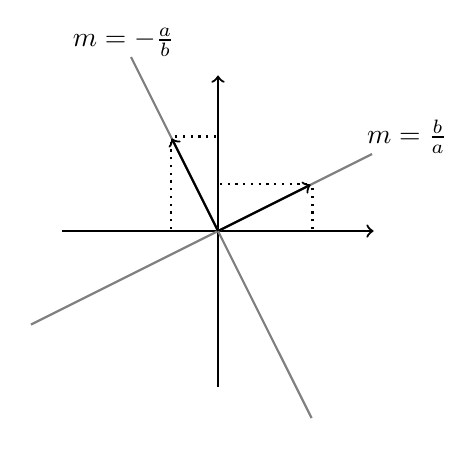
\begin{tikzpicture}
			    \node [inner sep=0pt] at (0, -2) (0) {};
			    \node [inner sep=0pt] at (2, 0) (1) {};
			    \node [inner sep=0pt] at (0, 2) (2) {};
			    \node [inner sep=0pt] at (-2, 0) (3) {};
			    \draw [black, thick, ->] (0) -- (2);
			    \draw [black, thick, ->] (3) -- (1);
			    
			    \node [inner sep=0pt] at (1.2, 0.6) (MP) {};
			    \node [inner sep=0pt] at (2.4, 1.2) (MPEF) {$m=\frac{b}{a}$};
			    \node [inner sep=0pt] at (-2.4, -1.2) (MPEB) {};
			    \draw [gray, thick] (MPEB) -- (MPEF);
			    \draw [black, thick, ->] (0,0) -- (MP);
			    \node [inner sep=0pt] at (1.2, 0) (MPA) {};
			    \draw [black, thick, dotted] (MPA) -- (MP);
			    \node [inner sep=0pt] at (0, 0.6) (MPB) {};
			    \draw [black, thick, dotted] (MPB) -- (MP);
			    
			    
			    \node [inner sep=0pt] at (-0.6, 1.2) (MN) {};
			    \node [inner sep=0pt] at (-1.2, 2.4) (MNEF) {$m=-\frac{a}{b}$};
			    \node [inner sep=0pt] at (1.2, -2.4) (MNEB) {};
			    \draw [gray, thick] (MNEB) -- (MNEF);
			    \draw [black, thick, ->] (0,0) -- (MN);
			    \node [inner sep=0pt] at (0, 1.2) (MNA) {};
			    \draw [black, thick, dotted] (MNA) -- (MN);
			    \node [inner sep=0pt] at (-0.6, 0) (MNB) {};
			    \draw [black, thick, dotted] (MNB) -- (MN);
		    \end{tikzpicture}\\
		
		    $U = Span (\Set{u})$\\
		    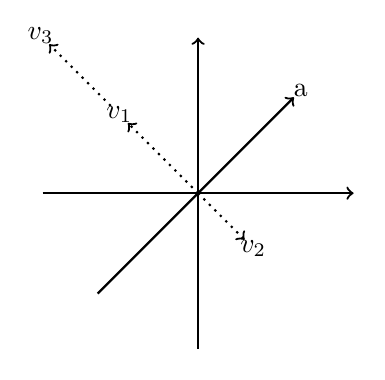
\begin{tikzpicture}
			    \node [inner sep=0pt] at (0, -2) (0) {};
			    \node [inner sep=0pt] at (2, 0) (1) {};
			    \node [inner sep=0pt] at (0, 2) (2) {};
			    \node [inner sep=0pt] at (-2, 0) (3) {};
			    \draw [black, thick, ->] (0) -- (2);
			    \draw [black, thick, ->] (3) -- (1);
			    
			    \node [inner sep=0pt] at (1.3, 1.3) (AP) {a};
			    \node [inner sep=0pt] at (-1.3, -1.3) (AN) {};
			    \draw [black, thick, ->] (AN) -- (AP);
			    
			    \node [inner sep=0pt] at (0.7, -0.7) (v2) {$v_2$};
			    \node [inner sep=0pt] at (-1, 1) (v1) {$v_1$};
			    \node [inner sep=0pt] at (-2, 2) (v3) {$v_3$};
			    \draw [black, thick, dotted, ->] (0,0) -- (v2);
			    \draw [black, thick, dotted, ->] (0,0) -- (v1);
			    \draw [black, thick, dotted, ->] (v1) -- (v3);
		    \end{tikzpicture}\\
	    
	\ssect{Definition: Orthogonalraum}
	    Sei V ein euklidischer $\bR$-VR mit Skalarprodukt $\circ$ und u sei UVR von
	    V.
	    \ilmath{U^\bot = \Set{v \in V \mid \forall u \in U: v \circ u = 0}}
	    heißt \underline{Orthogonalraum} (orthogonales Komplement) zu U in V.
	
	\ssect{Bemerkung}
	    $U^\bot$ ist ein UVR von V.
	    \paragraph{Beweis}
	    \begin{enumerate}
	        \item $0_V \in U^\bot$, denn: $0_V \in V \checkmark$
	        \ilmath{\underbrace{0_V \circ u}_{\in \bR} = (0_v + 0_v) \circ u = 0_v \circ u + 0_v \circ u \implies 0 = 0_v \circ u}
	        
	        \item $u_1, u_2 \in U^\bot \implies u_1 + u_2 \in U^\bot$, denn: $u_1 + u_2 \in V$
	        $(u_1 + u_2) \circ u = u_1 \circ u + u_2 \circ u = 0 \checkmark$
	
	        \item $v \in U^\bot, r \in \bR \implies r v \in U^\bot$, denn
	        $rv \in V$, $rv \circ u = r(\underbrace{v \circ u)}_{= 0} = 0$ für alle $u \in U \checkmark$
	    \end{enumerate}
	    
	    V VR, U, $U^\bot$ UVR.
	\ssect{Bemerkung: Gemeinsamkeiten $U$ und $U^\bot$}
	
	    $U \cap U^\bot = \Set{0_v}$
	    \ilmath{v \in U \cap U^\bot \implies v \in U \cap v \in U^\bot \implies v \circ v = 0 \implies v = 0_v}
	\ssect{Bemerkung: dim mit Orthogonalräumen}
	 
	    \ilmath{dim V = dim U + dim U^\bot}
	
	    \paragraph{Beispiel}
	    $V = \bR^3, U = span (\Set{u_1, u_2})$
	
	    \ilmath{U^\bot = span (\Set{u_3})}
	
	\ssect{Berechnung von Orthogonalräumen}
	    u gegeben durch Basis.
	    
	    \paragraph{Bem}
		    Sei $U = span (\Set{b_1, b_2, \ldots, b_k})$, sei $v \circ b_1 = \ldots = v \circ b_k = 0$
		    Dann:
		    \ilmath{v \circ (r_1 b_1 + \ldots, r_k b_k) = v \circ r_1 b_1 + \ldots + v \circ r_k b_k = \\
		     r_1 \underbrace{(v \circ b_1)}_{= 0} + \ldots + r_k \underbrace{(v \circ b_k)}_{= 0} = 0}
		
	    \paragraph{Beispiel}
		    \ilmath{U = Span (\Set{\ve{1}{1}{1}, \ve{1}{2}{3}}) \text{UVR von } \bR^3}
		    ges $U^\bot$
		
		    \ilmath{\ve{x}{y}{z} \in U^\bot \iff \ve{x}{y}{z} \in \bR^3 \land \ve{1}{1}{1} \circ \ve{x}{y}{z} = 0 \land \ve{1}{2}{3} \circ \ve{x}{y}{z} = 0}
		    
		    \ilmath{U^\bot = ker (A) = Row (A)^\bot}
		    \ilmath{Ker (A^\bot) = Col (A)^\bot}
	
	\ssect{Definition: Orthogonalbasis}
	    Sei V ein eukl. $\bR$-VR und $\Set{b_1, b_2, \ldots, b_k}$ eine Basis von V.
	    $\Set{b_1, b_2, \ldots, b_k}$ heißt Orthogonalbasis, wenn gilt:
	    \ilmath{b_i \circ b_j = 0 \text{für alle } i, j \in \Set{1, \ldots, k} \land i \neq j}
	    \paragraph{Beispiel} 
		    \begin{enumerate}
		        \item Standartbasis ist eine Orthogonalbasis
		        \item $\Set{\ve{1}{1}{0}, \ve{1}{-1}{0}, \ve{0}{0}{1}}$ ist eine Orthogonalbasis des $\bR^3$
		    \end{enumerate}
		
	\ssect{Satz}
	    Sei $\Set{b_1, \ldots, b_k}$ eine Orthonormalbasis von V, $v \in V$
	    
	    Dann gilt: $v =(\star) r_1 b_1 + \ldots + r_i b_i + \ldots + r_k b_k$ mit $\boxed{r_i = \frac{v \circ b_i}{b_i \circ b_i} = v \circ b_i}$
	    
	
	    $\star$ mit $b_i$ mult. bzgl. Skalarprodukt.
	    \ilmath{v \circ b_i = (r_1 b_1 + \ldots + r_i b_i + \ldots + r_k b_k) \circ b_i \implies v \circ b_i = r_i (b_i \circ b_i)}
	   
	\ssect{Definition: Orthonarmalbasis}
	    Sei $\Set{b_1, \ldots, b_k}$ eine Orthogonalbasis von V. 
	    $\Set{b_1, b_2, \ldots, b_k}$ heißt \underline{Orthonormalbasis}, wenn gilt:
	    \ilmath{|| b_i || = 1 \text{ für } i = 1, \ldots, k}
	    
		\ilmath{ \left|\left|\frac{b_i}{||b_i||}\right|\right| &= \sqrt{\frac{b_i}{||b_i||} \circ \frac{b_i}{||b_i||}} \\
		    &= \sqrt{\frac{1}{||b_i||^2} b_i \circ b_i} \\ 
		    &= \frac{1}{||b_i||} \sqrt{b_i \circ b_i} = 1}
		\ilmath{b_i \circ b_i = || b_i ||^2 = 1}
\end{document}
